\documentclass{article}
\usepackage{graphicx}
\usepackage{authblk}
\usepackage{amsmath}


\begin{document}
\title{THEORETICAL NEUROSCIENCE \\ EXERCISE 5}
\date{\today}
\author[1]{\c{S}eyma Bayrak\thanks{seyma.bayrak@st.ovgu.de}}
\affil[1]{\footnotesize  Otto von Guericke University of Magdeburg}
\maketitle

\section{Introduction}
Hodgkin and Huxley experimented quid giand axon and demonstrated consequently the analysis of action potential at neuron. The Hodgkin-Huxley (HH) model depens basically on single compartment model (SCM) with leak conductance and ion conductances of $Na^+$ and  $K^+$. The particularity of HH model relies on the crucial propoerty of ion conductances: The conductance changes under varying membrane potential, $V_{m}$, and time parameter.  \\

What defines the conductance of an ion channel? The answer is that, the fraction of open or closed channels for a specific type of ion determines the membranes conductance for this specific ion. Opening-closing rate of channels are symbolized with three letters: "m, n, h". \textbf{m} and \textbf{n} are the activation variables for the m and n gates for $Na^+$ ion, and \textbf{h} is the activation variable for the h gates for $K^+$ ion. Those fractions change in time by varying $V_{m}$. In the computational part of this assignment, the calculation of activation variables will be mentioned in detail.\\

Now, let us start with the SCM and tyr to reach the generalized equation of HH model for the $V_{m}$.

\begin{equation}
i_{e}=i_{c}+i_{r}, \,\,\,\,\,\,\,\,\,\,\, i_{r}=i_{Na^+}+i_{K^+}+i_{L}, \,\,\,\,\,\,\,\,\,\,\,i_{m}=c_{m}\frac{dV_{m}(t)}{dt}  
\end{equation}
The current is the expression of conductance and potential difference. The current values of $Na^+$, $K^+$ ions and leak are presented below. Note that the conductance of leak is constant.
\begin{equation*}
i_{L}=g_{L}.(V_{m}-E_{L}),\,\,\,\,\,\,\,\,\,\,\,\,
\end{equation*}

\begin{equation*}
i_{Na}=g_{Na}(V,t).(V_{m}-E_{Na}),\,\,\,\,\,\,\,\,\,\,\,\,where\,\,\,\,g_{Na}(V,t)=\bar{g}_{Na}.m^3.h.
\end{equation*}

\begin{equation*}
i_{K}=g_{K}(V,t).(V_{m}-E_{K}),\,\,\,\,\,\,\,\,\,\,\,\,where\,\,\,\,g_{K}(V,t)=\bar{g}_{K}.n^4
\end{equation*}
When the current expressions given above are inserted in equation 1, a very long and unlikely equation is reached as seen by equation 2. 
\begin{equation}
 c_{m}\frac{dV_{m}(t)}{dt}=i_{e}-g_{L}.(V_{m}-E_{L})-\bar{g}_{Na}m^{3}h(V_{m}-E_{Na})-\bar{g}_{K}n^4(V_{m}-E_{K})
\end{equation}
 The purpose is now to re-formulate the equation 2 and get a "SCM looking like" version. Following mathematical tricks can be examined for this purpose. 
\begin{equation*}
 c_{m}\frac{dV_{m}(t)}{dt}=i_{e}+g_{L}E_{L}+\bar{g}_{Na}m^{3}hE_{Na}+\bar{g}_{K}n^4E_{K}
\end{equation*}

\begin{equation*}
\,\,\,\,\,\,\,\,\,\,\,\,\,\,\,\,\,\,\,\,\,\,\,\,\,\,\,\,-V(g_{L}+\bar{g}_{Na}m^{3}h+\bar{g}_{K}n^4) \,\,\,\,\,\, \Longrightarrow
\end{equation*}

\begin{equation*}
 \frac{c_{m}}{(g_{L}+\bar{g}_{N
a}m^{3}h+\bar{g}_{K}n^4)}\frac{dV_{m}}{dt}=\frac{(i_{e}+g_{L}E_{L}+\bar{g}_{Na}m^{3}hE_{Na}+\bar{g}_{K}n^4E_{K})}{(g_{L}+\bar{g}_{Na}m^{3}h+\bar{g}_{K}n^4)}-V
\end{equation*}
At this point, it is crucial to define two new variables just by re-naming our old variables as the following below.
\begin{equation*}
 \tau_{eff}(t)=\frac{c_{m}}{(g_{L}+\bar{g}_{Na}m^{3}h+\bar{g}_{K}n^4)}
\end{equation*}

\begin{equation*}
 V_{\infty}^{eff}(t)=\frac{(i_{e}+g_{L}E_{L}+\bar{g}_{Na}m^{3}hE_{Na}+\bar{g}_{K}n^4E_{K})}{(g_{L}+\bar{g}_{Na}m^{3}h+\bar{g}_{K}n^4)}
\end{equation*}

\begin{equation}
 \Rightarrow\frac{dV_{m}(t)}{dt}=\frac{1}{\tau_{eff}}[V_{\infty}^{eff}(t)-V_{m}(t)]
\end{equation}
Eqaution 3 is a simpler-looking differential equation of $V_{m}$, it is also the reflection of SCM. It is important to emphasize that, activation (or gating) variables are always denoted by single letters \texttt{m, n, h} above, however, more scientific represantation would be \textit{m(V,t), n(V,t), h(V,t)}.Relevant differential equations are stated below.
\begin{equation}
 \frac{dm(V,t)}{dt}=-\frac{1}{\tau_{m}} [m(V,t)-m_{\infty}(V)]
\end{equation}

\begin{equation}
 \frac{dh(V,t)}{dt}=-\frac{1}{\tau_{h}}[h(V,t)-h_{\infty}(V)]
\end{equation}
\begin{equation}
 \frac{dn(V,t)}{dt}=-\frac{1}{\tau_{n}}[n(V,t)-n_{\infty}(V)]
\end{equation}

 \section{Programming Assignment}

The purpose of programming assignment is to define the membrane potential $V_{m}$ and the gating variables $m$, $n$, and $h$ by given parameters such as a time interval, an input current etc. All the  parameters are defined as below. \\

$
T=40 ms\,\,\,\,\,\,\ dt=0.1 ms\,\,\,\,\,\,\ i_{e}=0 nA/mm^2 \,\,\,\,\,\,\ c_{m}=10 nF/mm^2 $


$
E_{L}=-54.402 mV\,\,\,\,\,\,\,\,\,\,\,\,\,\ E_{Na}=50 mV \,\,\,\,\,\,\,\,\,\,\,\,\,\ E_{K}=-77 mV \,\,\,\,\,\,\  $

$
\bar{g}_{L}=3 \mu S/mm^{2}\,\,\,\,\,\,\,\,\,\,\,\,\,\ \bar{g}_{Na}=1200 \mu S/mm^{2}\,\,\,\,\,\,\,\,\,\,\,\,\,\ \bar{g}_{K}=360 \mu S/mm^2 \,\,\,\,\,\,\  $

$ V_{m}(t=0)=-70 mV \,\,\,\,\,\,\,\,\,\,\,\,\,\ m(t=0)=h(t=0)\,\,\,\,\,\,\,\,\,\,\,\,\,\ n(t=0)=0.3$ \\ 

The programming assignment is defined step by step below,\\

\setcounter{tocdepth}{1}
\textbf{1.} The provided MATLAB functions were used to find the vectors $m_{\infty}$, $\tau_{m}$, $n_{\infty}$, $\tau_{n}$, $h_{\infty}$, $\tau_{h}$. The each element of those six vectors all depend on $V_{m}$ and time, so they were calculated inside a \textit{loop}.

\setcounter{tocdepth}{1}
\textbf{2.} The calculated variables were set into equations 4,5,6. This time, those equations could be numerically solved to get the vectors of $m$, $n$, $h$. Note that, the initial values of gating variables play an important factor here. 

\setcounter{tocdepth}{1}
\textbf{3.} The computed gating variables were inserted into the formulas of $V_{\infty}^{eff}$ and $\tau_{eff}$.

\setcounter{tocdepth}{1}
\textbf{4.} The last step of programming assignment was to solve the differential equation of $V_{m}$ (stated by equation 3) numerically. The previous steps did already provided all unknown parameters for the integration.\\

The plotted graphs of changing $V_{m}$ and gating variables under time variance can be seen in graph 1. Additionally, the resting potential $V_{rest}$ of the simulated neruon is found to be -65.0034 mV.

\begin{center}
 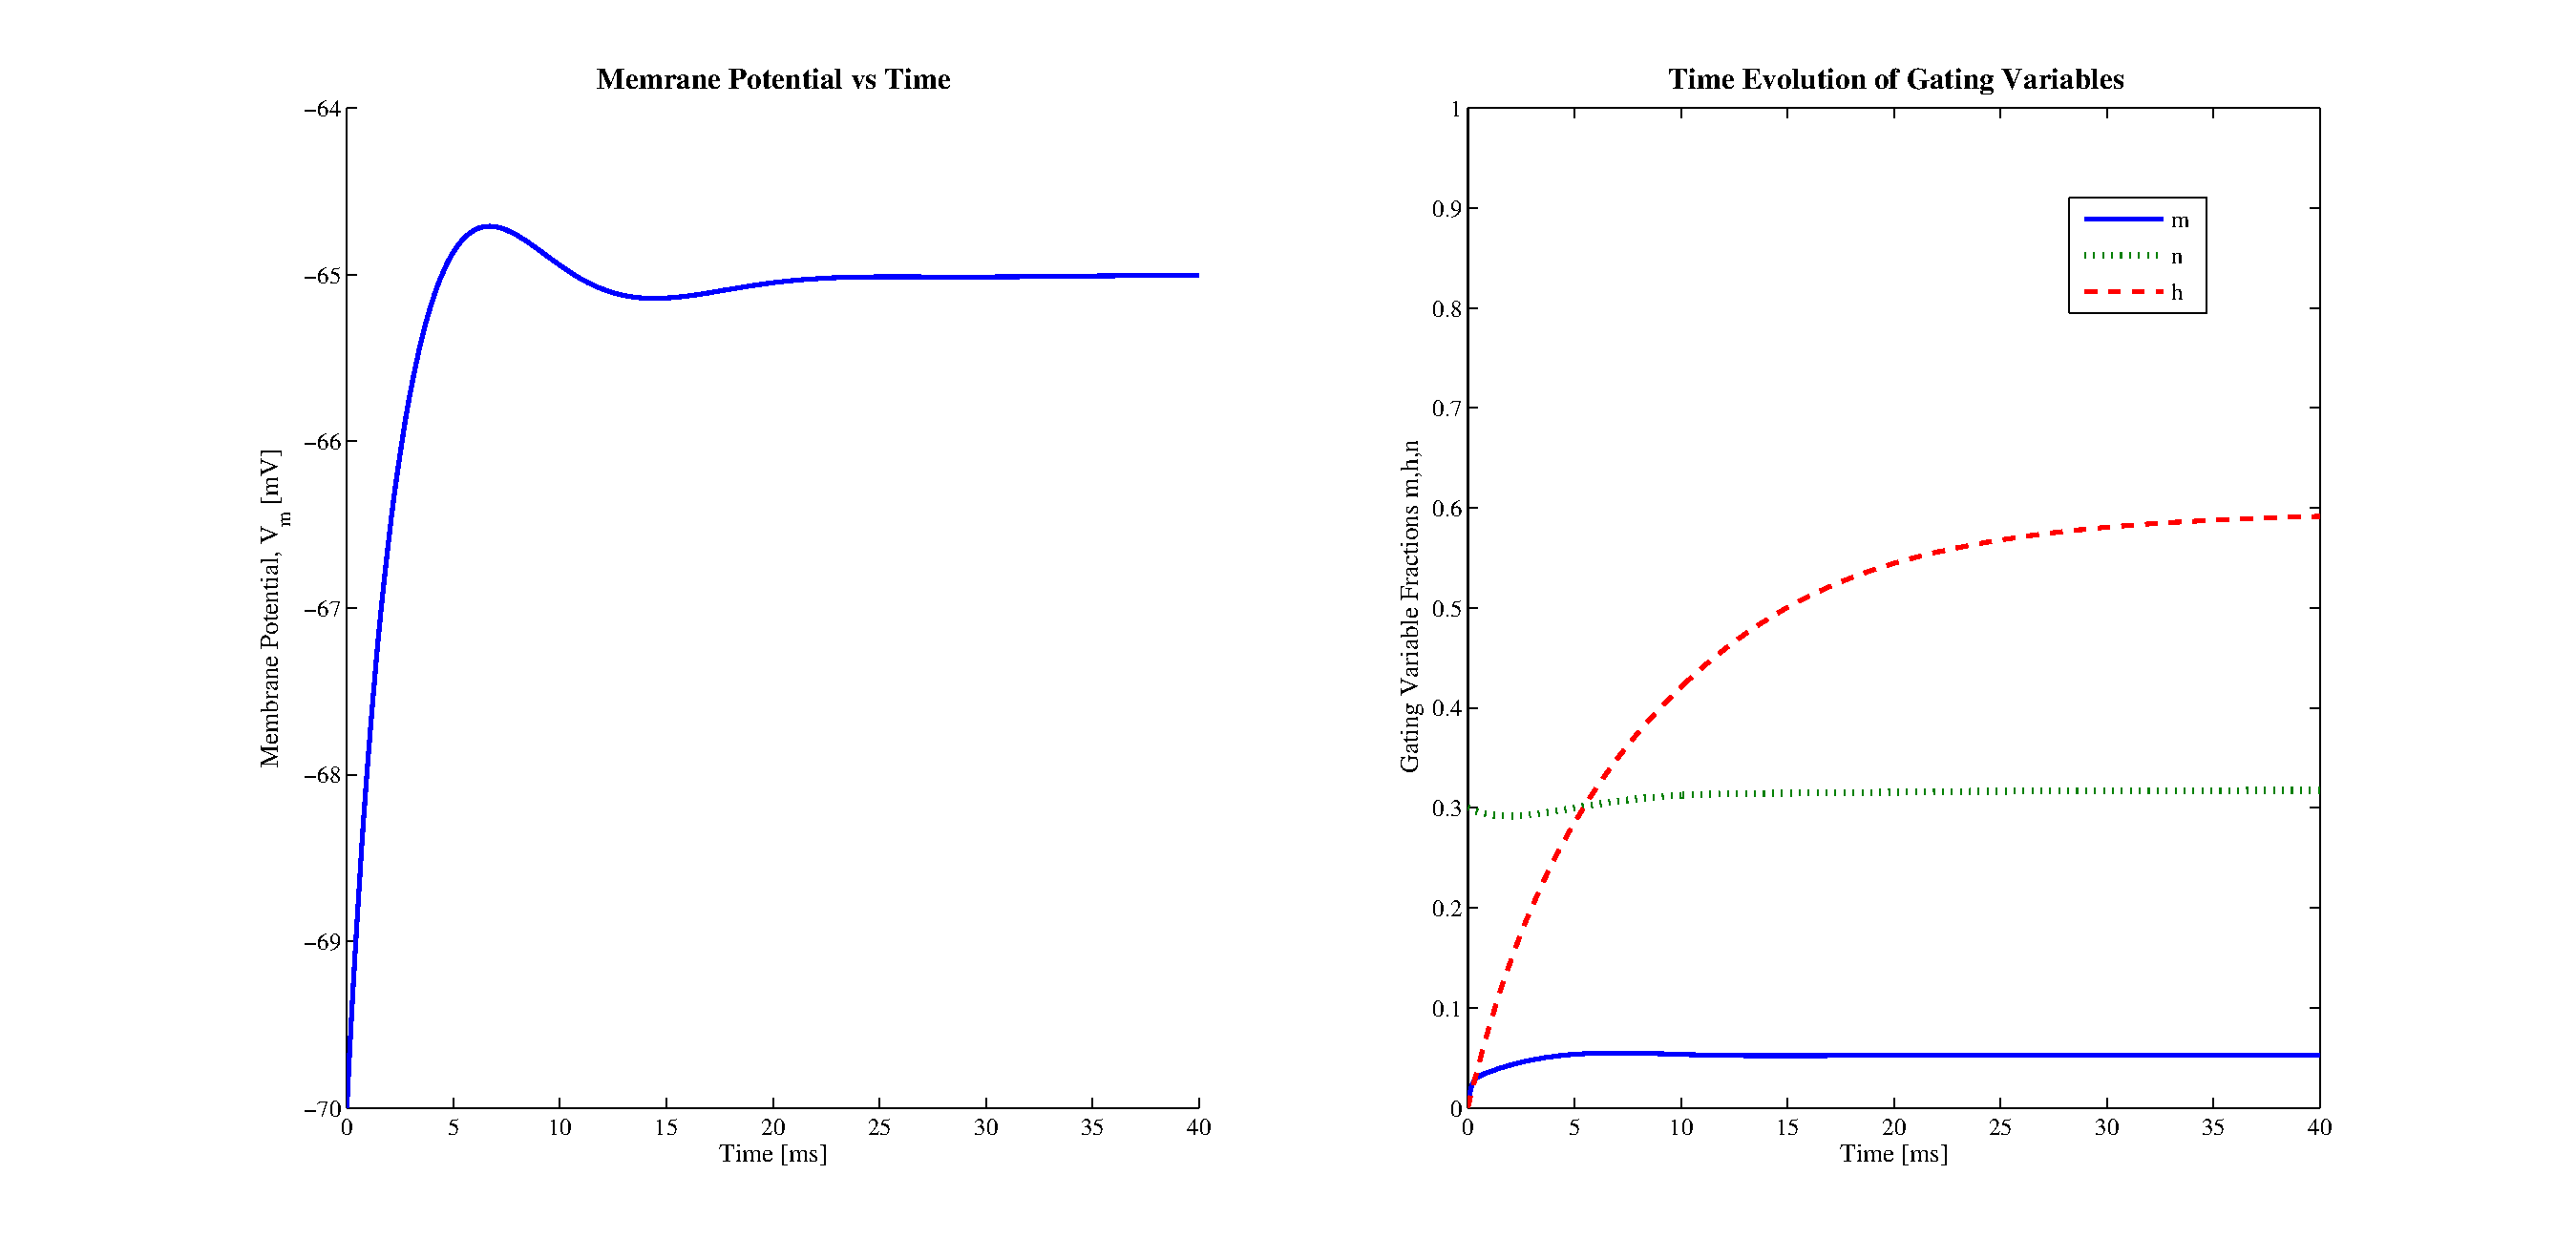
\includegraphics[width=\textwidth]{figur1.eps}
 % q7.eps: 0x0 pixel, 300dpi, 0.00x0.00 cm, bb=  -86   231   682   610
\begin{footnotesize}Graph 1, the left one is for $V_{m}$ and the right one is that of $m$, $n$, and $h$. \end{footnotesize}
\end{center}
\section{Discussion}
Our simulation indicates that, membrane potential depolarizes fastly from -70 mV to approximately -64.7 Mv at the very beginning of time interval. However, a certain hyperpolarization back to value around -65.1 mV is observed. The hyperpolarization is followed by a small increment to -65 mV. Then it stays almost constant at this value at the second half of time interval. This constant potential value is already defined as $V_{rest}$.\\

The rightest part of graph 1 shows that the biggest number of fraction of open gates belongs to $K^+$ channels. $m$ gates of $Na^+$ and $h$ gates of $K^+$ are assumed to be zero (closed) at t=0 ms; they increase then exponentially, but $h$ increases much faster. $n$ gates were defined at t=0 ms as the 3 \% of them are open (n(t=0)=0.3), the opening fraction of it also increases but the slowest compared to $m$ and $h$ gates. The common attitude of m, n, h is to relax to an equilibrium value after a certain time.\\ 

Now, let us try to analyze relation between $V_{m}$ and $m$, $n$, $h$. The effect of $K^+$ ion flux through the membrane is to push the $V_{m}$ value to $E_{K}=-77 mV$. On the other hand, $Na^+$ ions make the opposite by pushing $V_{m}$ up to $E_{Na}=50 mV$. At t=0, the n-gated Na channels are dominant to other gates, that is why depolarization occurs. After a short time, the most dominant gates are h gates; more than half of K channels are open! This causes the hyperpolarization at $V_{m}$. After all, the gate fractions reach more constant values, the net effect on $V_{m}$ is to stay at $V_{rest}$, but still more close to $E_{K}$.\\

Let us change some of our initially defined parameters, and observe the change on graphs. Time interval was expanded from 40 ms to 100 ms, and $n(t=0)$ was set to 0 this time. The graph 2 reflects those two changes.
\begin{center}
 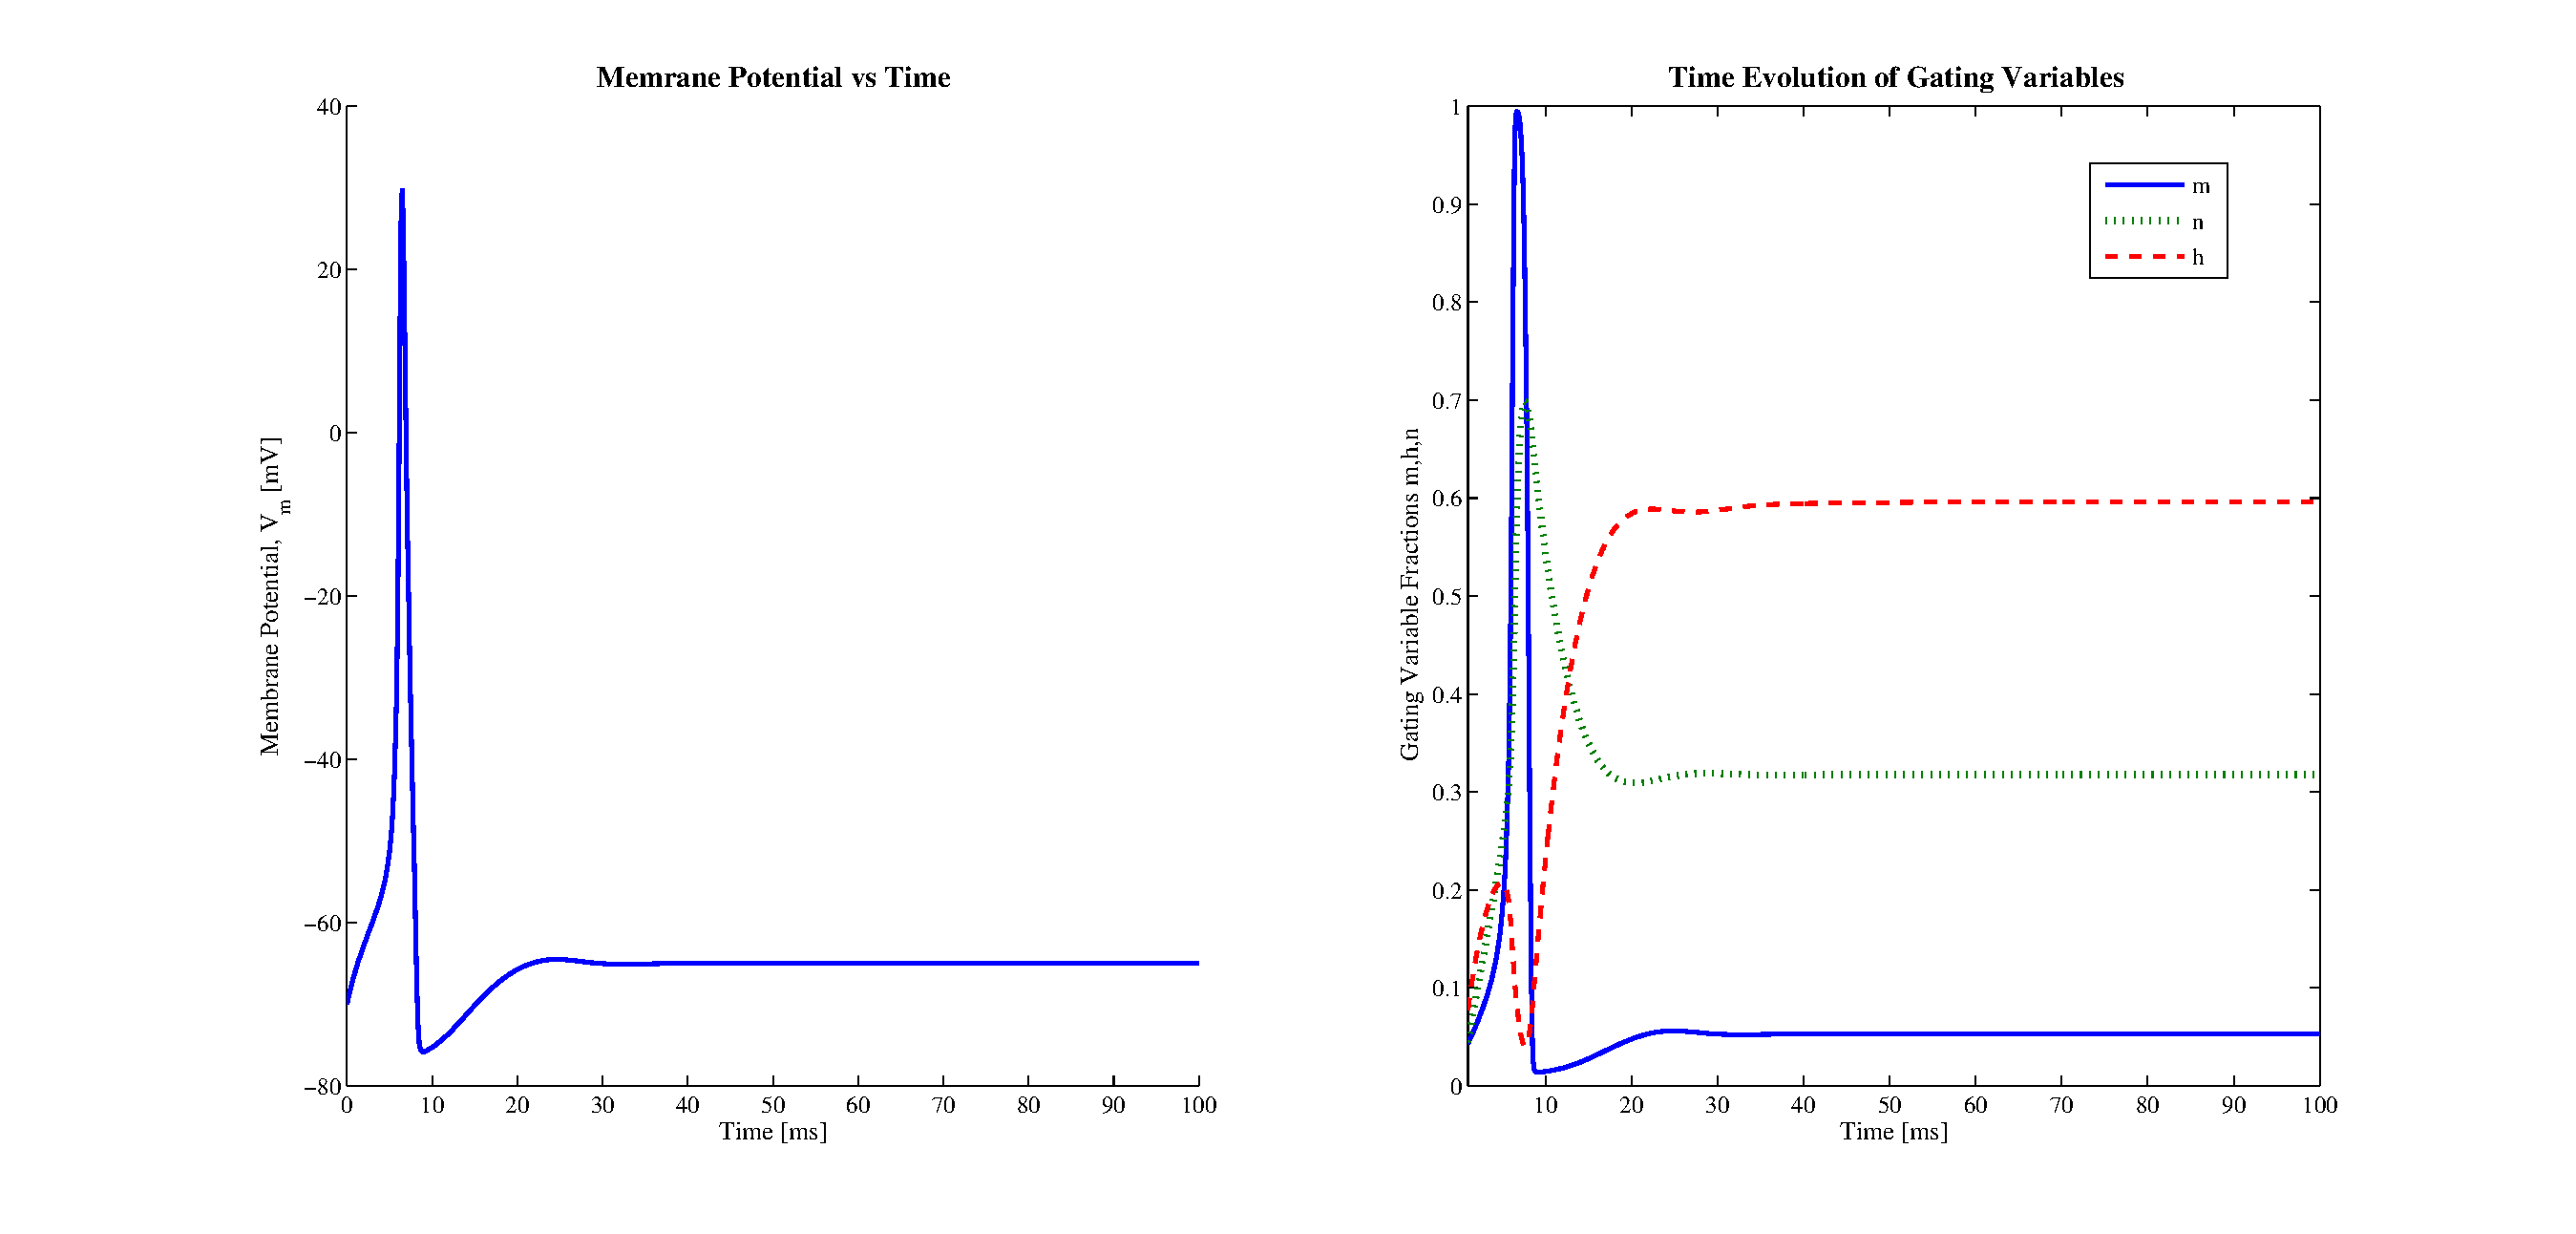
\includegraphics[width=\textwidth]{discus1.eps}
 % q7.eps: 0x0 pixel, 300dpi, 0.00x0.00 cm, bb=  -86   231   682   610
\begin{footnotesize}Graph 2, t=100 ms, $n(t=0)=0$ . \end{footnotesize}
\end{center}

Graph 2 indicates that m and n increase very dramatically, almost all of the m-gated Na channels seem to be open, This reflects itself as a rapid depolarization on $V_{m}$ up to around 30 mV; Na ions pushes it to be close to $E_{Na}=50 mV$. Then m and n decrease whereas h increases fastly . At the end m,n and h relax to constant values. h is the biggest fraction, therefore $V_{rest}$ is -65 mV. \\

Secondly, the input current was changed to the value of 100 $nA/mm^2$. The following graph is eliminated.

\begin{center}
 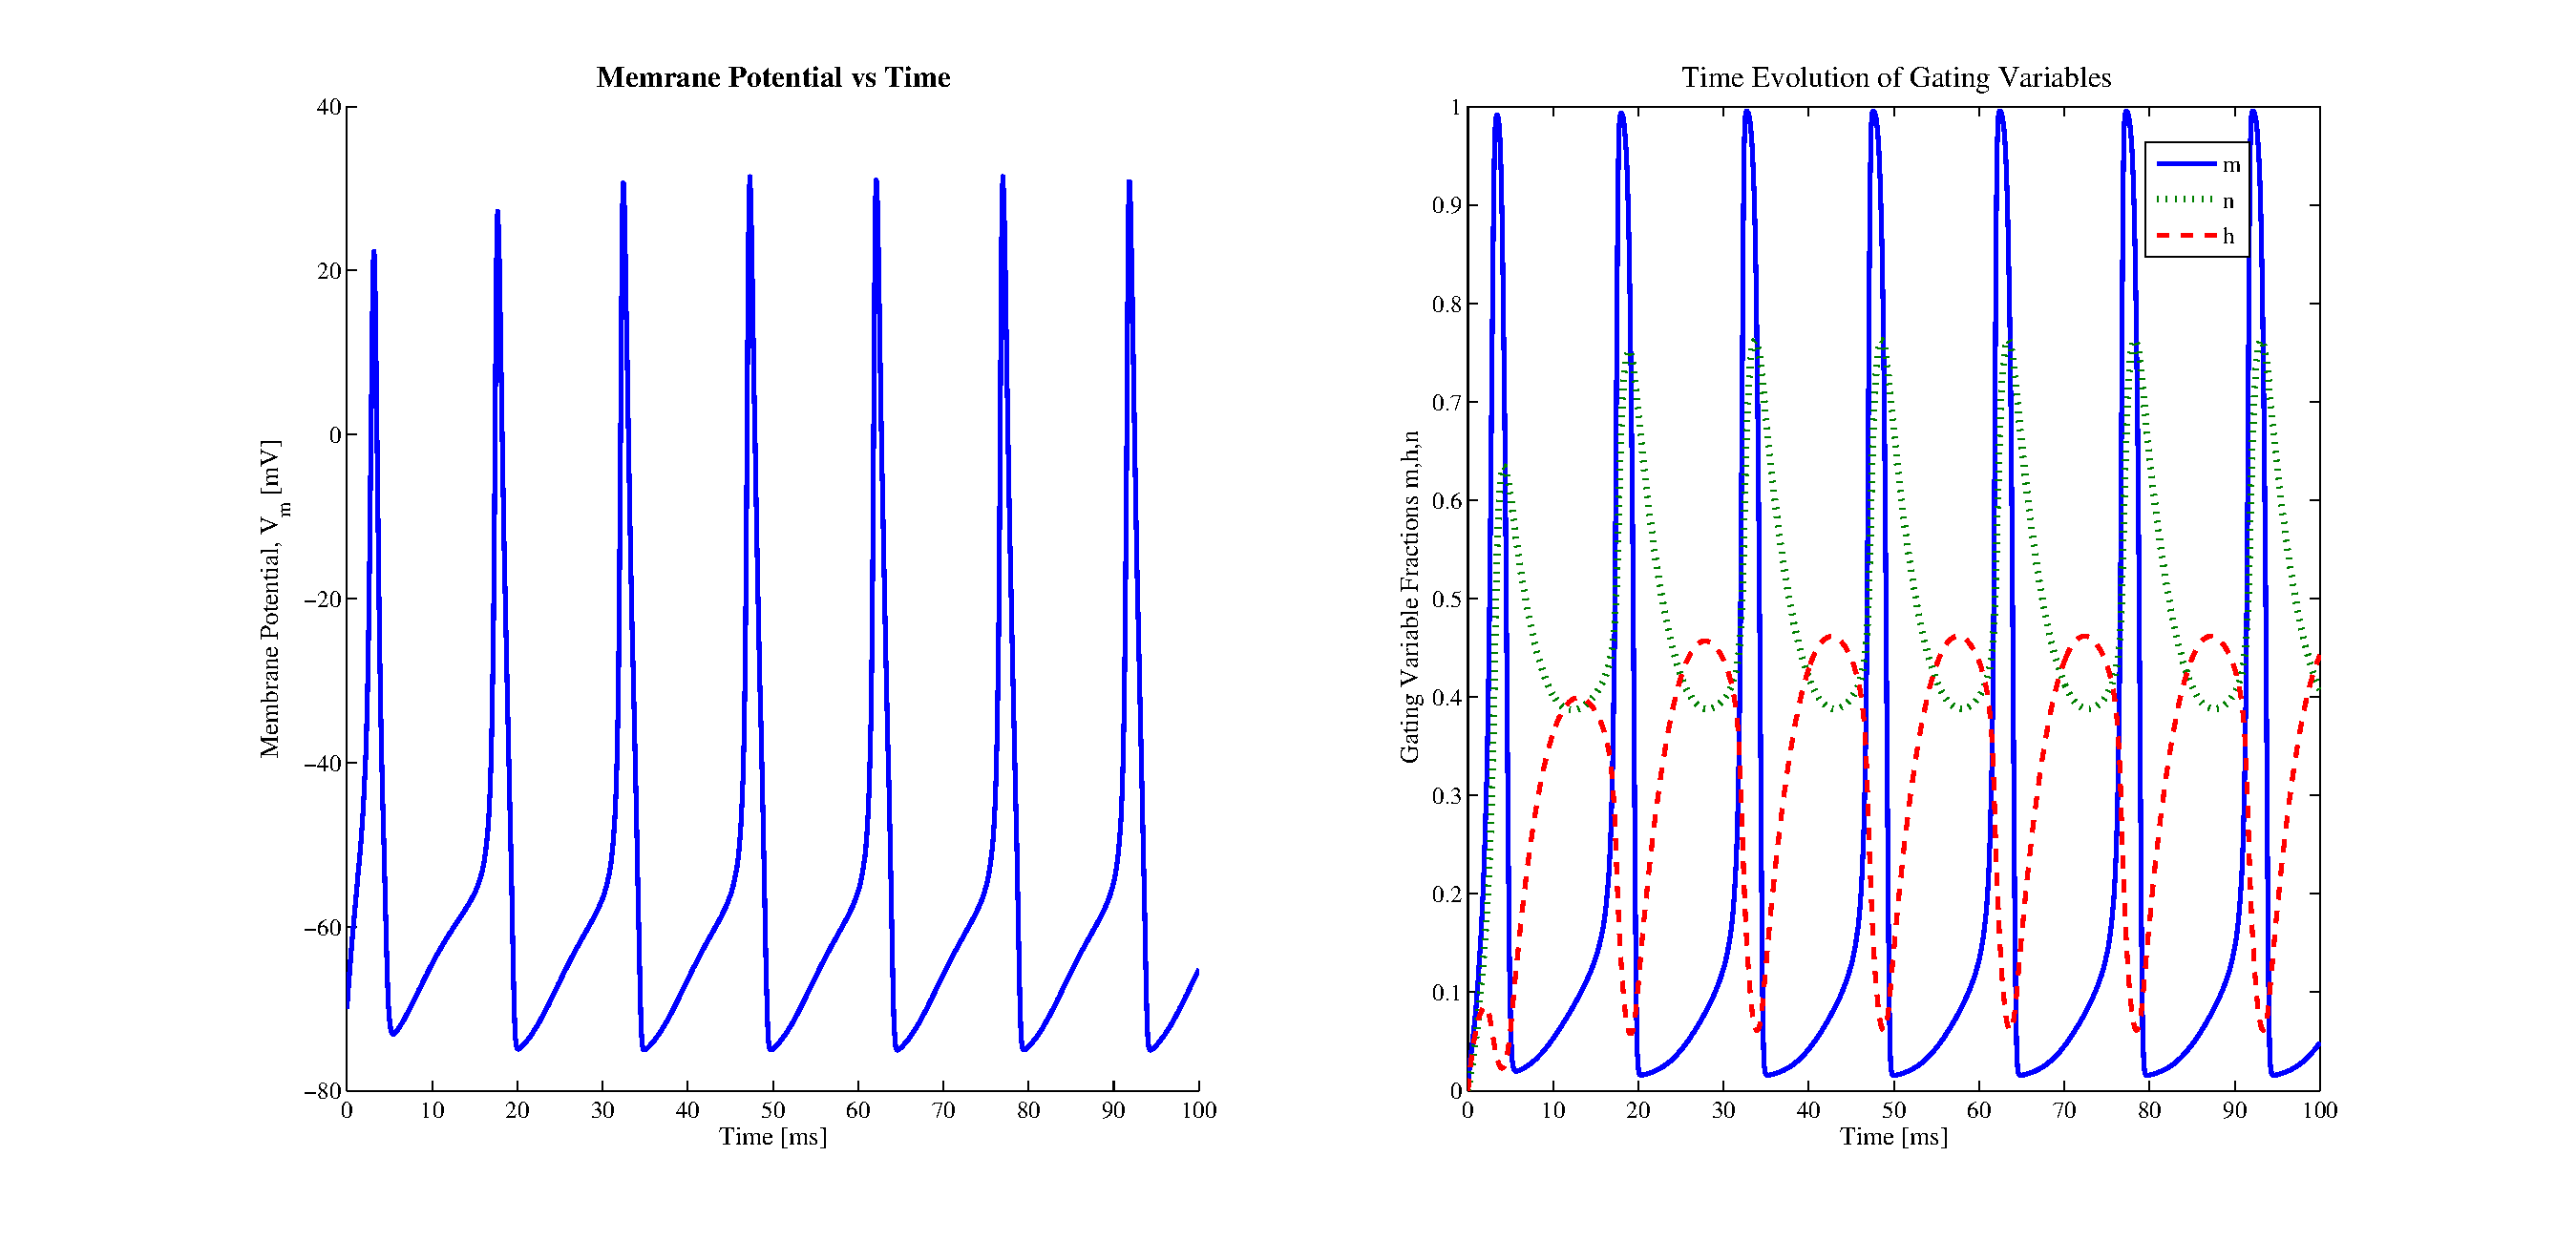
\includegraphics[width=\textwidth]{discus2.eps}
 % q7.eps: 0x0 pixel, 300dpi, 0.00x0.00 cm, bb=  -86   231   682   610
\begin{footnotesize}Graph 3, t=100 ms, $n(t=0)=0$, $i_{0}=100 nA/mm^2$  \end{footnotesize}
\end{center}

Graph 3 shows the fact that a very high increment in input current leads the "spikes" at $V_{m}$ - so called action potentials. Since the m and n gates become open faster than h gates at beginning, $V_{m}$ depolarizes up to almost 30 mV, which seems likely to be threshold potential. Then h becomes greater, therefore $V_{m}$ hyperpolarizes to $V_{reset}$, it equals to -76 mV, very close to K reversal potential value. These events occur subsequently in certain time intervals.\\

Thirdly, the input current was set to 65 $nA/mm^2$. The graph 4 on the next page shows the change.\\

This time the input current value is not enough to yield the subsequent action potential occurances at $V_{m}$ as the grapg 4 shows. Again, the rapid changes in m and n gates and following depolarization at $V_{m}$ could be observed. The main difference between graph 1 and graph 4 is that, there exist some "wavy" changes in gate variables and $V_{m}$, but then they all relax exponentially to constant values. $V_{rest}$ equals to almost -61 mV, the hyperpolarization is slightly more compared to previous graphs.\\

Finally, the initial value of franction of h-gated K channels was defined as 0.5; we assumed that half of the K cahnnels are open at the beginning, whereas m and n were assumed to be zero at t=0 ms. The input current is again 65 $nA/mm^2$. The resultant graph 5 can be seen on next page.

\begin{center}
 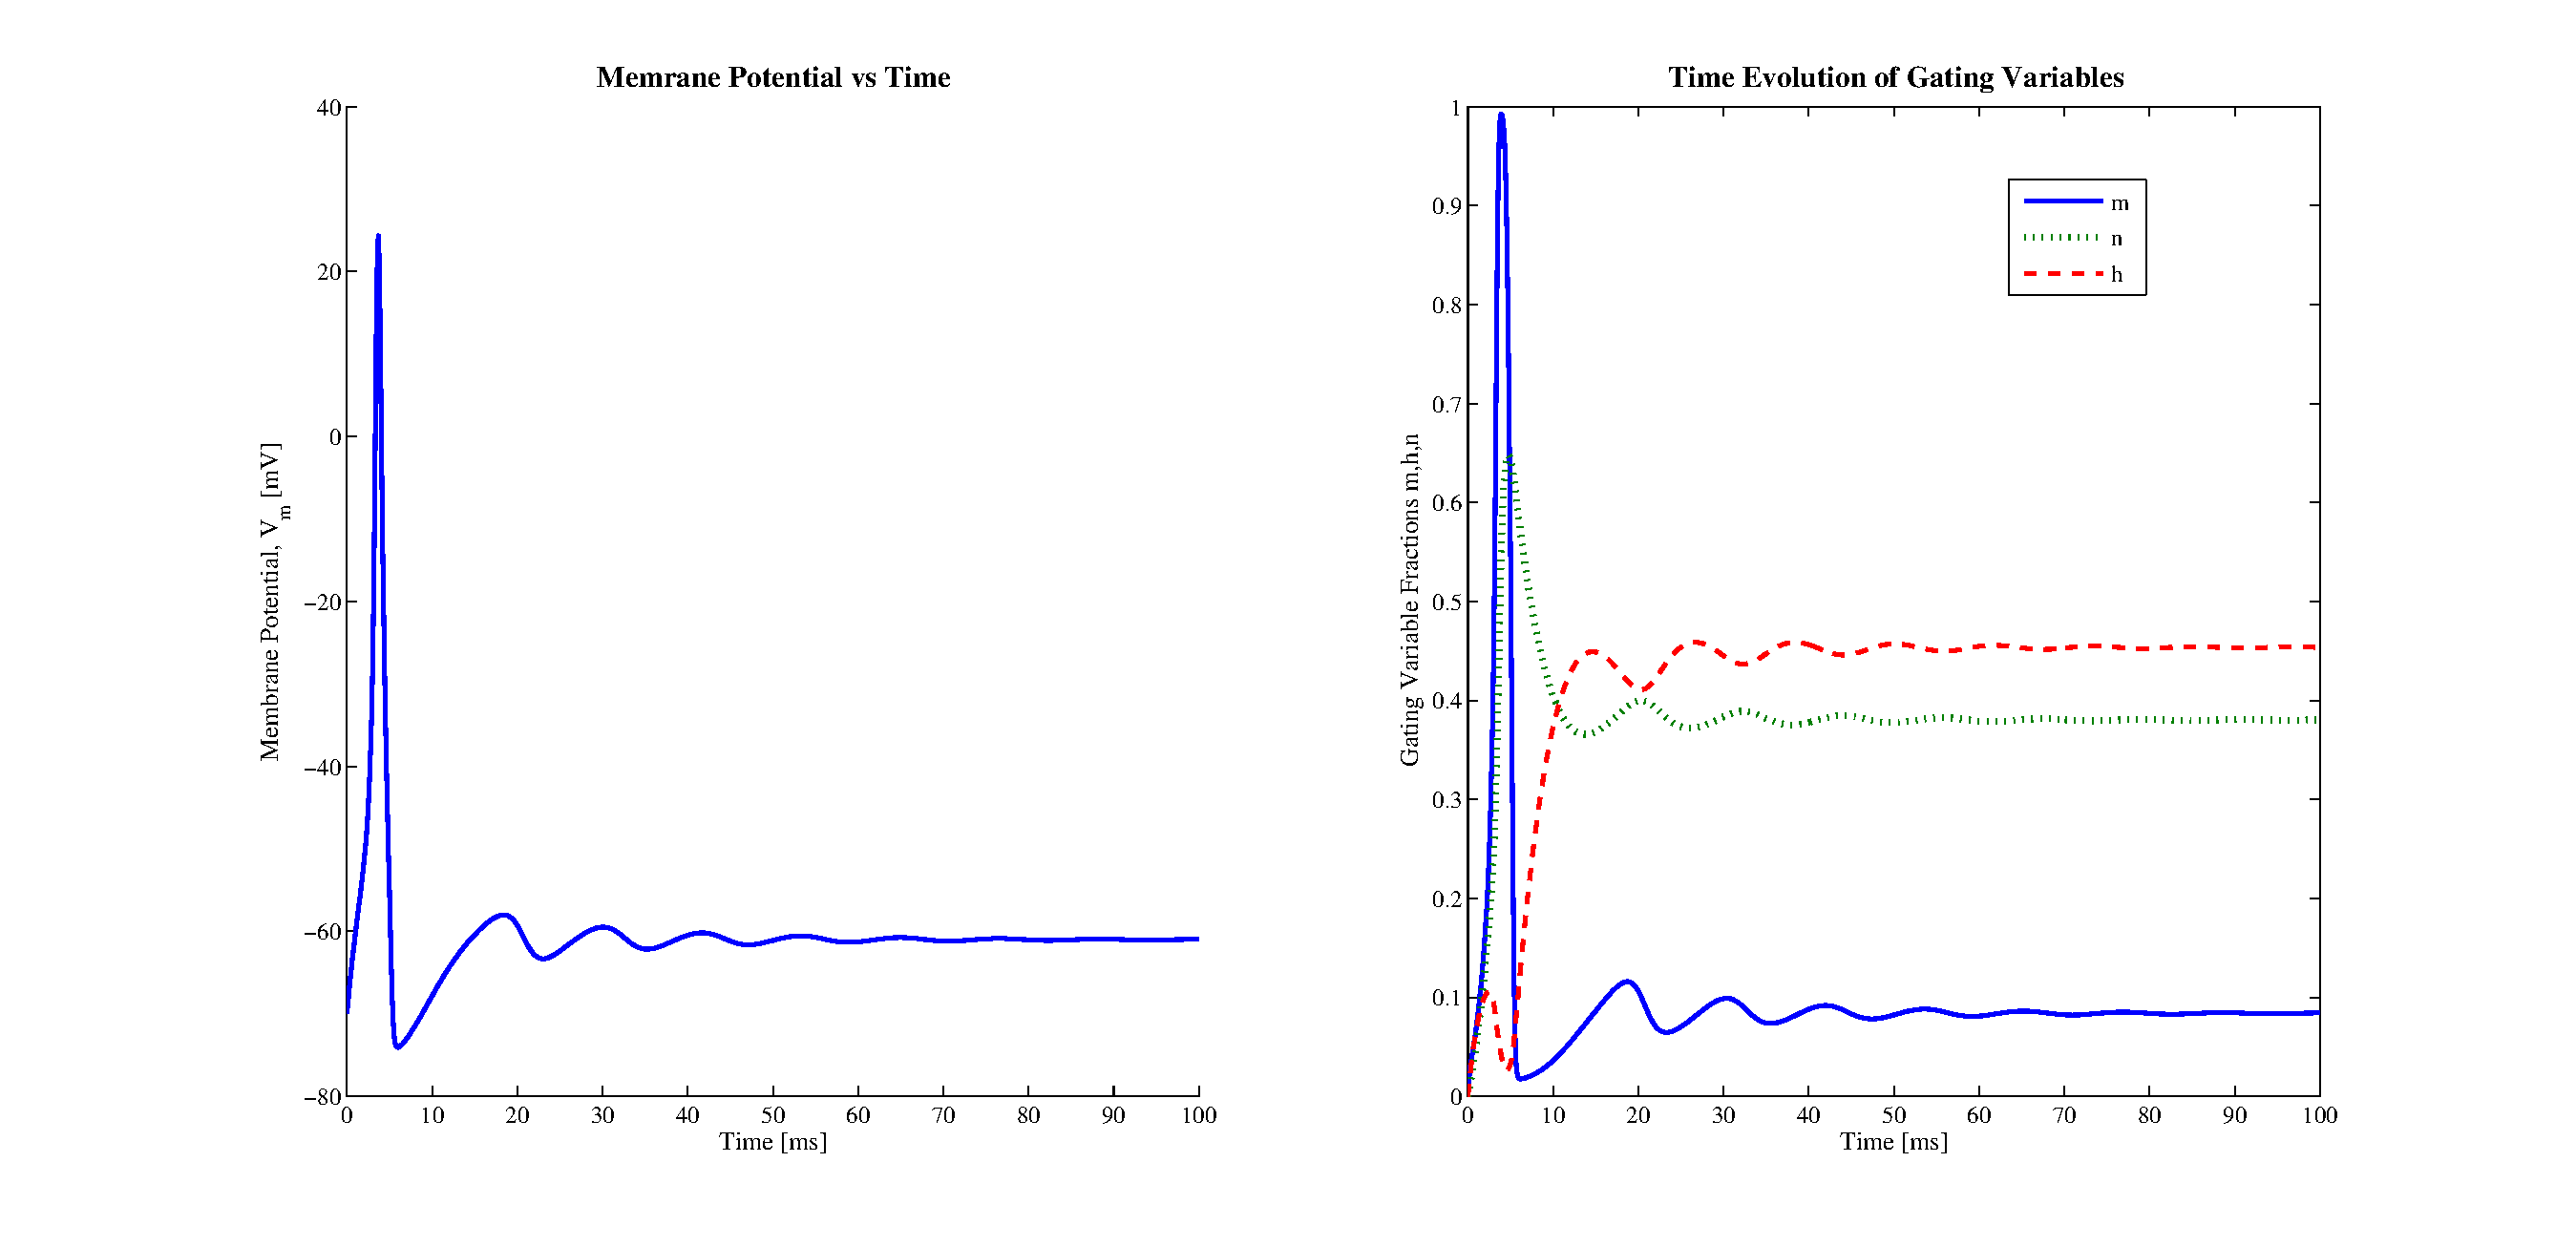
\includegraphics[width=\textwidth]{discus3.eps}
 % q7.eps: 0x0 pixel, 300dpi, 0.00x0.00 cm, bb=  -86   231   682   610
\begin{footnotesize}Graph 4, t=100 ms, $n(t=0)=0$, $i_{0}=65 nA/mm^2$  \end{footnotesize}
\end{center}

\begin{center}
 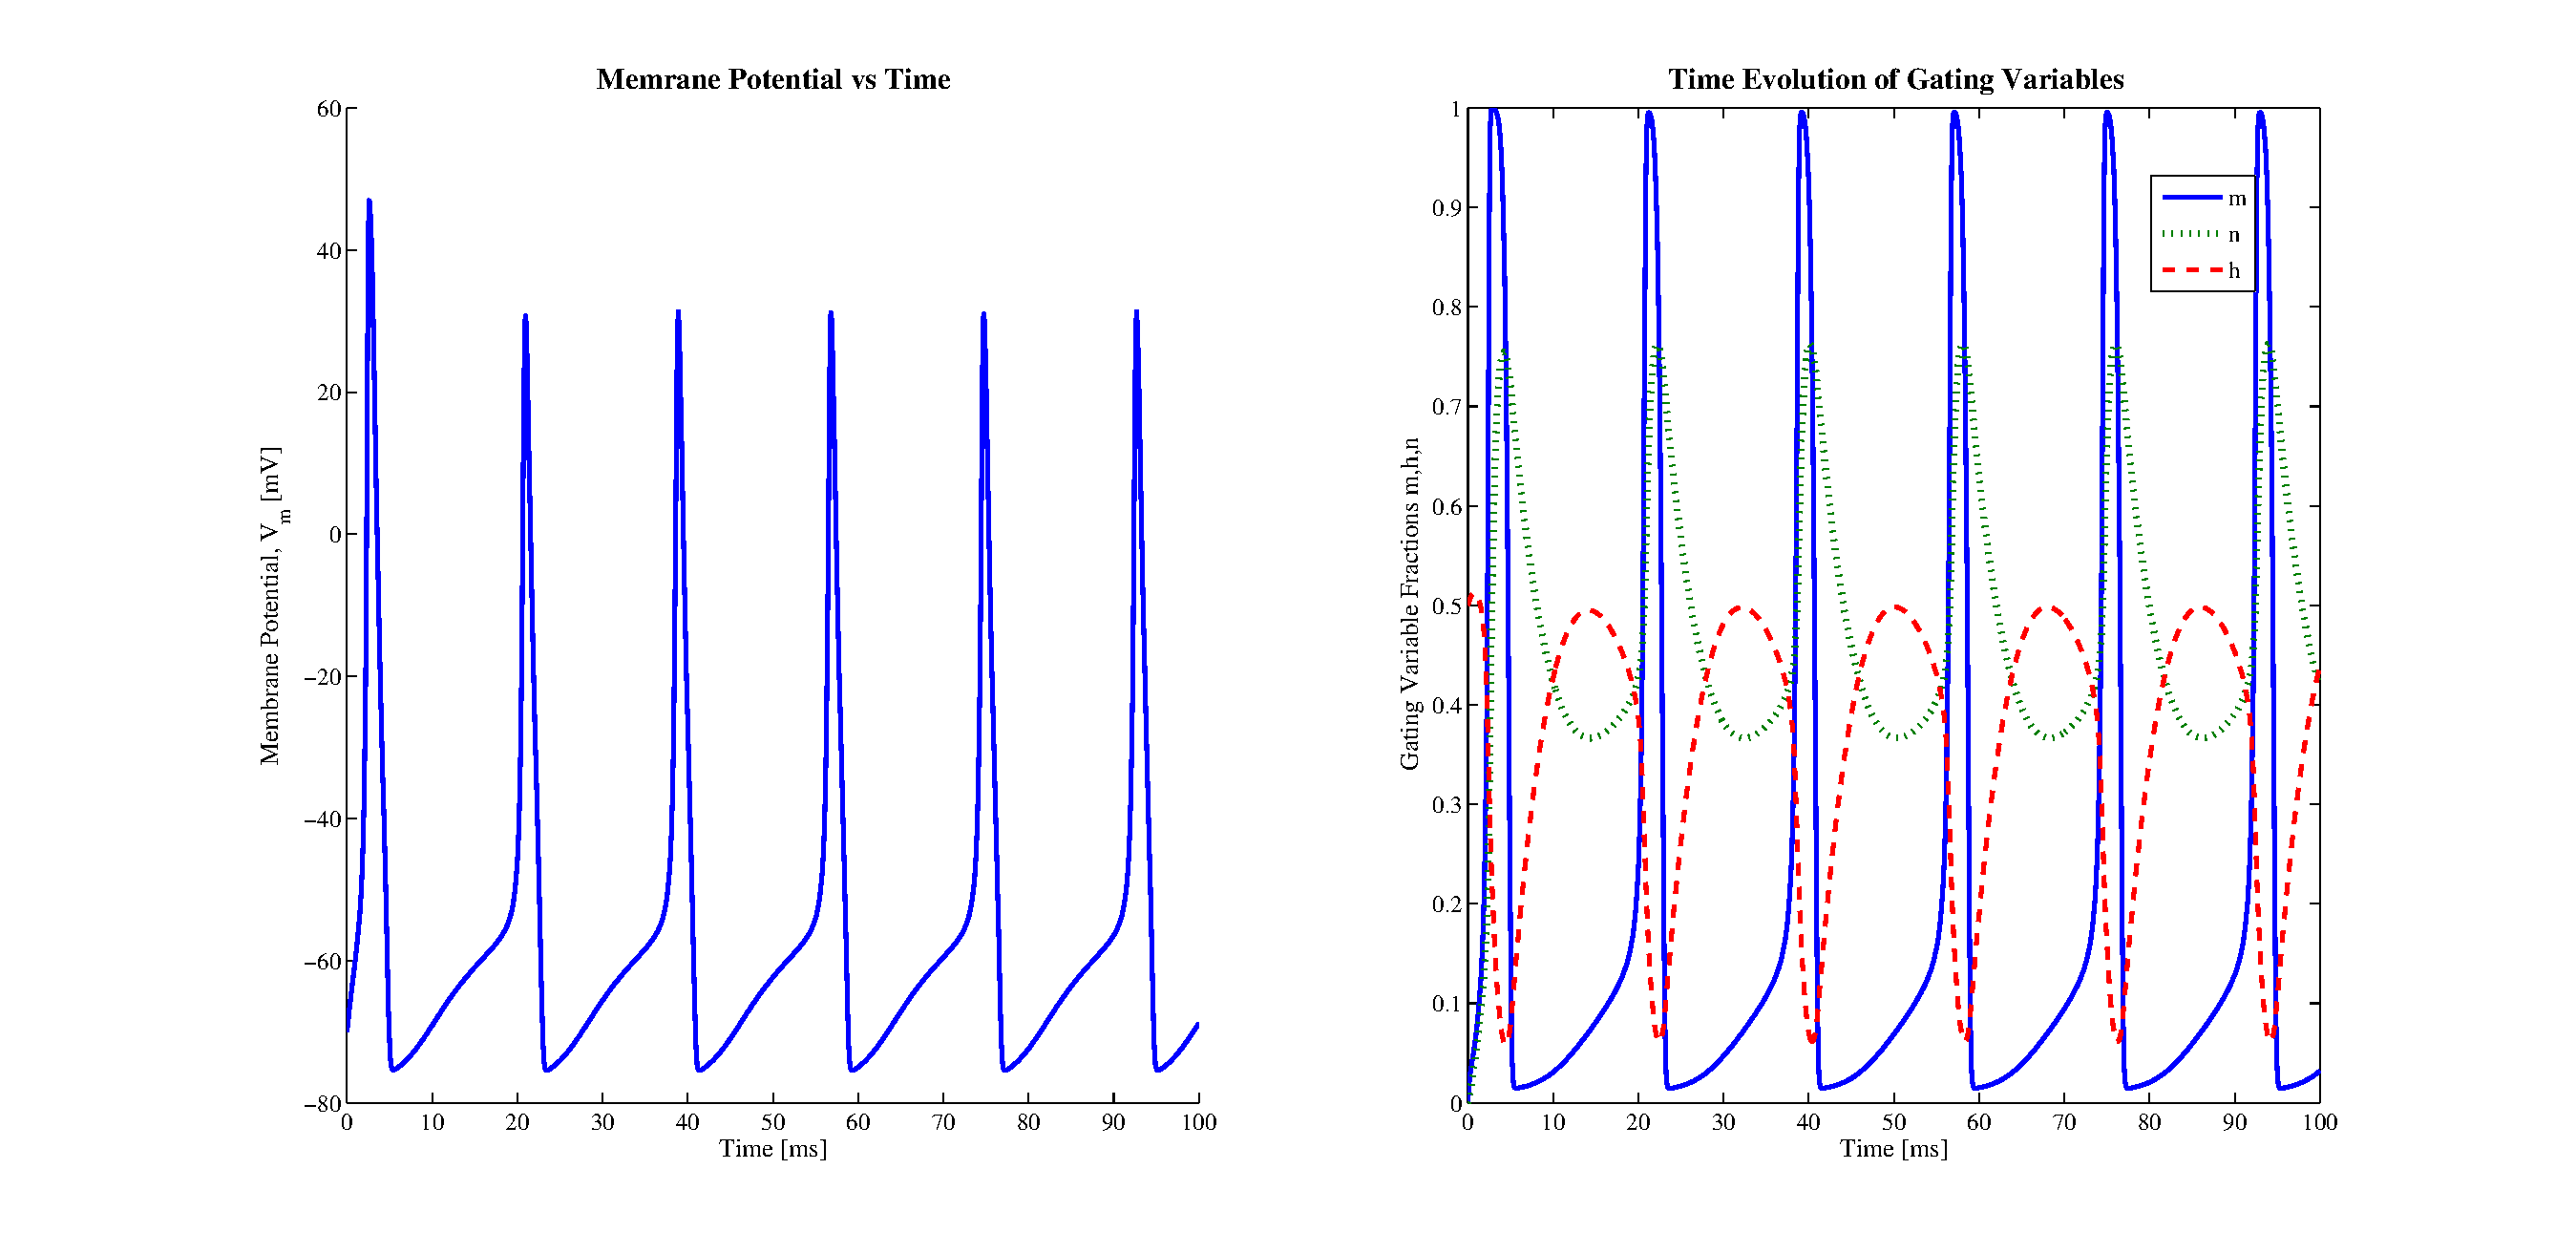
\includegraphics[width=\textwidth]{discus4.eps}
 % q7.eps: 0x0 pixel, 300dpi, 0.00x0.00 cm, bb=  -86   231   682   610
\begin{footnotesize}Graph 5, t=100 ms, $h(t=0)=0.5$, $i_{0}=65 nA/mm^2$  \end{footnotesize}
\end{center}

Graph 5 shows spikes at $V_{m}$. Even though current value is small compared to the graph 3, the 50 \% open h-gates at t=0 yields action potentials now. Graph 5 is highly identical to graph 3, same interpretations are also valid here, The value of $V_{rest}$ is barely around -76 mV, which is very close to $E_{K}=-77 mV$! \\ 

\end{document}
